\subsection{How tight is the bound?}\label{sec:tight}
We lifted the 40 test objects with grips 0--15\% below the no-onset grip, at three lift durations and three values of $r$,
and evaluated Proposition~\ref{prop:lift} with $r_{\max}$ equal to the true $r$ (Fig.~\ref{fig:tightness}). Three results
stand out. \textbf{The bound is loose}: among the 1{,}309 lifts with a non-zero bound in which the rod stayed in the grasp,
the median ratio of measured slip to bound was 0.023 (90th percentile 0.50). The probe's 0.9 step and the quasi-static
model's conservatism together leave most under-gripped lifts with little or no slip. \textbf{A zero bound meant no slip}:
the 360 lifts with a zero bound slipped at most 0.49\,mm, all of it creep. \textbf{The bound can be exceeded during long
slides}: 7 lifts, all at $T=1$\,s, $r=1$ and 3\% below the no-onset grip, slipped 26--44\,mm against a bound of 25\,mm. With
$r=1$ no friction switch is involved, so these slides expose a gap between the Coulomb model behind the bound and MuJoCo's
regularised sliding friction~\cite{todorov2012}. They do not affect the shield, which never certifies bounds of this size,
but they mark the limit of what the bound says about a simulated slide that lasts most of a second. The 491 lifts that
dropped the rod all had bounds above 12\,cm.

\begin{figure*}[t]\centering
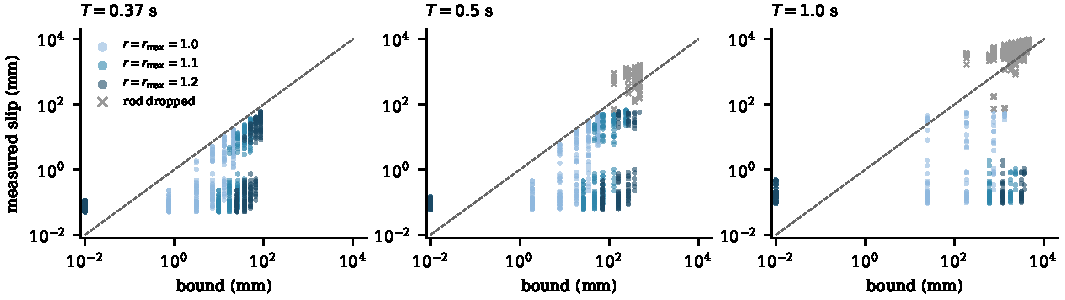
\includegraphics[width=\textwidth]{fig_tightness.pdf}
\caption{\textbf{Bound against measured slip} for deliberately under-gripped lifts (grip 85--100\% of the no-onset grip,
40 objects; log axes, zeros drawn at the left and bottom edges; dashed line: slip equal to the bound). Points below the line
are covered by the bound. Crosses are lifts that dropped the rod, where the slip is the rod's fall.}\label{fig:tightness}
\end{figure*}
